
\documentclass[a4paper]{report}
\renewcommand{\chaptername}{}
\usepackage{graphicx}


\begin{document}
%cover page

\titlepage 
\begin{center}
\huge\textbf{MagPY}\\[.5cm]
\LARGE\textnormal{(A Simplified Web Data Extraction System)}\\[.5cm]
\vspace{0.5cm}
\includegraphics[width=5.0cm]{logo.png}\\[0.7cm]
\vspace{.5cm}

\LARGE\textbf{MAIN PROJECT REPORT}\\[0.7cm]
\LARGE\textnormal{Submitted by}\\[0.5cm]
\Large \textbf {PAUL JACOB V}\\[.5cm]
\Large \textbf {SARATH S. MENON}\\[.5cm]
\Large \textbf {THUMSSY P. NAZAR}\\[1.5cm]


\large\textbf{Department of Computer Science and Engineering}\\[0.5cm]
\textbf{Rajagiri School of Engineering and Technology}\\[0.5cm]
\textbf{Rajagiri Valley, Kakkanad, Kochi, 682039}\\[0.5cm]
\textbf{APRIL 2015}\\[0.5cm]
\end{center}

\newpage
\begin{center}
\thispagestyle{empty}
\pagestyle{empty}
\large\textbf{RAJAGIRI SCHOOL OF ENGINEERING AND TECHNOLOGY}\\[.3cm]
\normalsize\textbf{RAJAGIRI VALLEY,KAKKANAD,KOCHI-39}\\[.6cm]
\vspace{.5cm}

\includegraphics[width=5.0cm]{Logo.png} \\[.7cm]
\vspace{.5cm}
\large\textbf{CERTIFICATE}\\[.5cm]
\end{center}
\large\textit{Certified that this is a Bonafide Record of the Main Project Report on }
\large\textit{\textbf{MagPY:A Simplified Web Data Extraction System }}
\large\textit{done by }
\large\textit{\textbf{Paul Jacob V, Sarath S Menon, Thumssy P.Nazar }}
\large\textit{with University Register Numbers }
\large\textit{\textbf{11012351,11012367,11012380 }}
\large\textit{of branch }
\large\textit{\textbf{Computer Science and Engineering }}
\large\textit{during the semester Eight year 2015 at Rajagiri School of Engineering and Technology,Kakkand,Kochi.}\\[2.0cm]

\large\textit{\noindent Project Guide \hfill Project Coordinator \hfill Head of the Department}


\newpage
\begin{center}
\fontsize{16.28pt}{19.2pt}
\textbf{ABSTRACT}\\[0.1cm]
\end{center}
\pagenumbering{roman}
\setcounter{page}{2}
\addcontentsline{toc}{chapter}{Abstract}

\paragraph{}
\large\textnormal{MagPY is a constraint based web data extractor, developed based on web scraping and web crawling. The Magpy is a project aimed at bringing about a better web search experience by providing a constraint based search rather than the simple keyword based approach as done by popular search engines like Google, Yahoo and Bing. The constraints are of different type, including negation of some words, size limit for the result, repetitions, regular expressions etc. Also, with a system to watch a web page for certain updates and with the ability to provide data from just targeted section of the page, MagPY improves the speed, accuracy and reduces the burden of the user to a large extent. }
\paragraph{}
\large\textnormal{In brief, this project is focused on producing a web based document extraction tool presented in a simple GUI, and provides the capabilities to search using keywords and regular expressions, and along with it, constrain the results based on different criteria. It acts as an advancement over the modern search engines by providing the capability to filter results and partial load web pages for contents or peek into the web pages, which is not possible in the current scenario.}
\paragraph{}
\large\textnormal{Taking into consideration the working of present search engines and crawlers, they work on the basis of the metadata like description, tags, SEO tips and keywords that are provided by the website creator. This can be a disadvantage if “keyword stuffing” or similar technique is used to fool the search engine, and be on top of their results. But MagPy does the job of further drilling down into the page and filtering the real and fake pages out. This project has got application in various domains like research, data mining, marketing etc. This project is going to be developed in Python and will run on platforms like Windows and Android}

\newpage
\begin{center}
\fontsize{17.28pt}{19.2pt}
\textbf{ACKNOWLEDGEMENT}\\[.5cm]
\end{center}
\pagenumbering{roman}
\setcounter{page}{3}
\addcontentsline{toc}{chapter}{Acknowledgement}
%\vspace{.cm}
\paragraph{}
\linespread{1.3}
\large\textnormal{A special gratitude to our final year project guide, Mr. Jayarajan J. N, Assistant Professor , whose contribution in stimulating suggestions and encouragement, helped us to coordinate our project especially in writing this report. He has assisted us through the entire project by providing the required modifications in each stage and evaluating continuously so that we could attain our target in right time.}

\paragraph{}
\large\textnormal{ We also thank our lab in-charge Ms. Mary Priya Sebastian, Assistant Professor, for her guidance and provided us with all support inside our lab. We thank our Mini Project in-charge Mrs. Gopika S, Assistant Professor, for giving timely instructions during the entire journey of our project. We have to appreciate the guidance given by other supervisor as well as the panels especially in our project presentation that has improved our presentation skills thanks to their suggestions and advices. We also thank other lab in-charge teachers namely Fr. Jaison Paul Mulerickal, Assistant Professor and Dr. John Jose, Assistant Professor too. We also thank the head of the institution Dr. A. Unnikrishnan , Principal and the head of the department Mr.Ajith S, Assistant Professor for all your support and co-operation.}

\paragraph{}
\large\textnormal{The entire project was made possible by providing us with the required machines and software’s by our college lab staffs, we thank them too. Furthermore we would also like to acknowledge our college and department of computer science for all their support and providing us with the required facilities.}
\tableofcontents

\newpage
\pagenumbering{arabic}
\setcounter{page}{1}

\chapter{Introduction}
\section{Problem Statement}
\paragraph{}
\large\textnormal{The main aim is to design a simplified web data extraction and processing system by providing capabilities to navigate through multiple web pages, collect relevant data, process it and export it into user-specified formats. It also aims at the ability to filter search results using various constraints, watch website updates and automate web based activities and to change the way users search for content in the web. }
\paragraph{}
\large\textnormal{Current web search experience experiences a lot of drawbacks including the
inability to use constraints in the search results, like to negate a keyword, limit the size of results, or to provide only results having a specified size, target only specific region of the result page rather than loading the whole page for viewing just a small portion of it and so on.With this project, we aim at removing all these limitations and provide a much better, simple, efficient, fast and fluidic experience in web search.}
\section{Project Scope/ Objective}
\paragraph{}
\large\textnormal{MagPy is a constraint based web document extractor, a project aimed at bringing about a better web search experience by providing a constraint based search rather than the simple keyword based approach as done by popular search engines like Google, Yahoo and Bing. The constraints are of different type, including negation of some words, size limit for the result, repetitions, regular expressions
etc. Also, with a system to watch a webpage for certain updates and with the ability to provide data from just targeted section of the page, MagPy improves the speed, accuracy and reduces the burden of the user to a large extent.}
\paragraph{}
\large\textnormal{In brief, this project is focused on producing a web based document extraction tool presented in a simple GUI, and provides the capabilities to search using keywords and regular expressions, and along with it, constrain the results based on different criteria. It acts as an advancement over the modern search engines by providing the capability to filter results and partial load web pages for contents or peek into the web pages, which is not possible in the current scenario.}
\paragraph{}
\large\textnormal{Comparing our proposed system to the existing one, we can highlight a few examples from google.Let us consider the case where a user wants a small article on some general topic, say “global warming”. When the user searches Google, he gets the following response:}
\vspace{0.1cm}
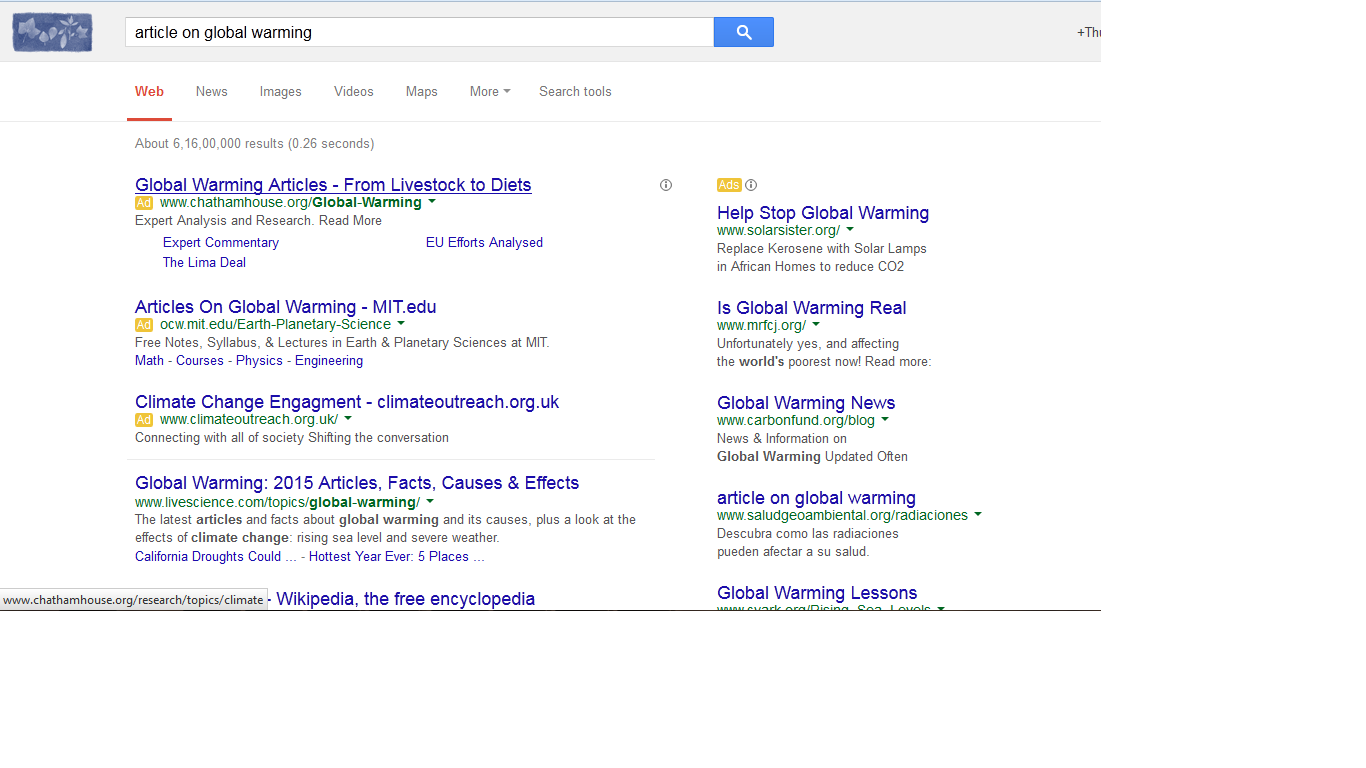
\includegraphics[width = 5in]{1.png} 
\vspace{0.1cm}
\paragraph{}
\large\textnormal{Instead of an article, he gets a list of links which contains contents related to the keyword, in this case, global warming. But It can be noticed that the first few links are ads, and also in certain cases, these links might not exactly contain what we want, for example, some may be false links, some may contain just a few lines, and some may be locked contents. We attempt to reduce such problems by extracting the content, checking whether they meet the user’s requirements, and displaying them instead of 
showing the links as shown. Another case would be the one related to negation of words. Suppose we want contents that do not contain a word or a set of words or maybe there would be cases where we specify negation to specify what we intend to mean, like using “kingfisher” as keyword and negating airlines refers to king fisher bird, but we get a result as follows:}
\vspace{.1cm}
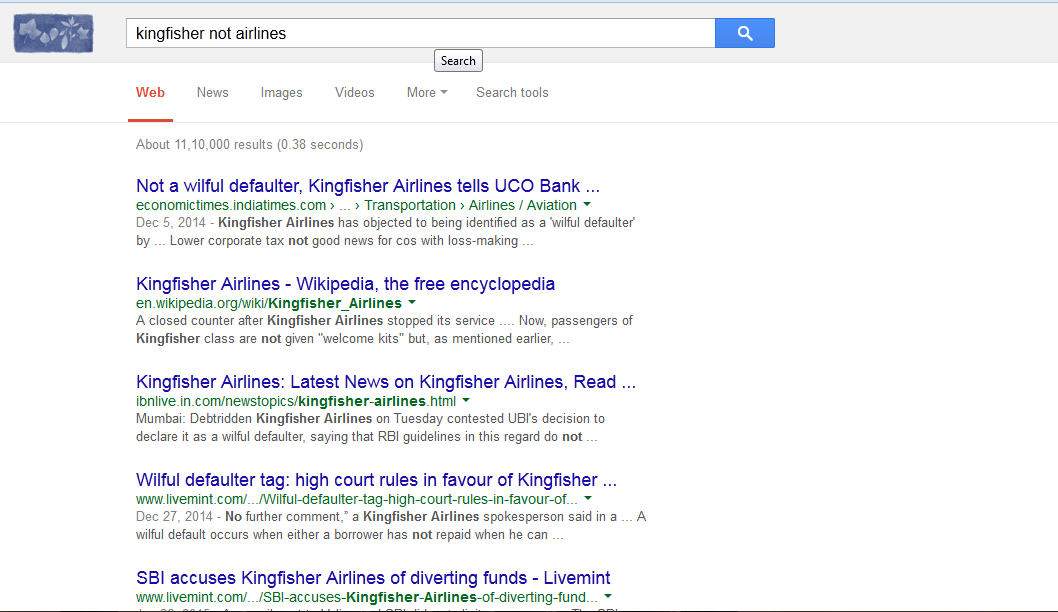
\includegraphics[width = 5in]{2.png} 
\vspace{.1cm}
\paragraph{}
\large\textnormal{Instead of filtering out airlines, it displays content only related to airlines! In order to highlight partial loading, we take the following examples. But under this category, we can notice that search engines like Google has advanced their engines towards this approach, so we just intend to provide some additional functionality to this. Let us consider the example of searching the answer to a question, say “Name of the highest peak in the world”. In google, the result is as follows:}

\vspace{0.3cm}
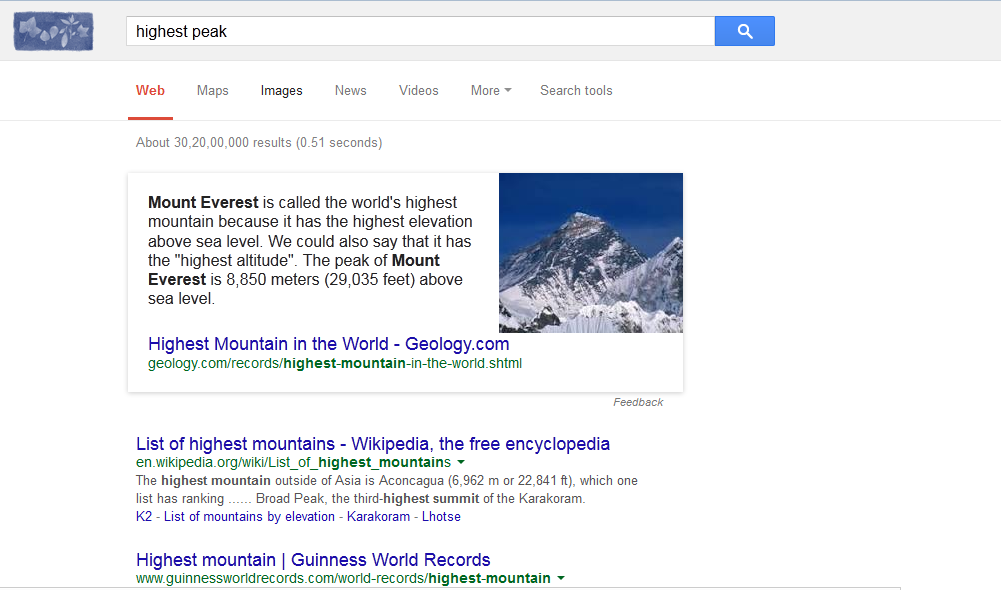
\includegraphics[width=5in]{3.png} 
\vspace{0.1cm}

\section{Design and Implementation Constraints}
\paragraph{}
\large\textnormal{This project involves an application front-end that needs to be simple and user friendly, as well as support all major platforms available. This is an important constraint due to the number of platforms that are present now. Another constraint is a good internet connection, as scraping web data involves large amount of data to be transferred, in a short time. But since most of the load of getting data from various websites and processing it is taken by the server, to the user, network usage would not be much of a limitation. Additionally, because of the inbuilt partial-load feature, data usage would be minimal in the long run. We are based on APIs provided by search engines like Google, Yahoo and 
Bing. So interfacing those APIs would be the next, but a minor design issue. Any minor changes issued by the providers of various APIs would cause faults in the system and might need a re-setup of the system for successful working again.Next issue is the storage requirement on the server side. Multiple user 
requests involve a large amount of websites to be scrapped, and a lot of data in involved in its processing. This would mean a server with large dynamic memory, and advanced enough to handle multi-threaded programming. Also since the system is built using Python, the server should support Python, which 
can be managed by using Django based server.}

\section{Assumptions and Dependencies}
\paragraph{}
\large\textnormal{This project utilizes data obtained from a large number of web sources,and hence has large dependencies. But since the initial step of selecting the top data sources is done by top and advanced search engines like Google and Yahoo, the possibility of erroneous sources is reduced, and we can safely assume that the data obtained is authentic, irrespective of the sources and the queries.Another important dependency arises due to the use of APIs provided by various providers, though they won’t bring out sudden, unnoticed changes, there should be a watch on the limitations and updates done to the APIs in the long run. However, we have planned a system that would make the system comparatively immune to API changes, thus reducing effects on the actual system.}

\section{Development Method}
\paragraph{}
\large\textnormal{For the development of this project, we have chosen the Agile Development strategy, mainly because it is comparatively more advanced than the older models and it lays more focus on doing than talking and documenting, thus improving the quality of the projects. Agile Project Management is one of the revolutionary methods introduced for the practice of project management. This is one of the latest 
project management strategies that is mainly applied to project management practice in software development. Though there were many existing development models for software engineering, more flexible software development models were required in order to address the agility of the requirements. As a result of this, the information technology community developed agile software development models.'Agile' is an umbrella term used for identifying various models used for agile development, such as Scrum. Since agile development model is different from conventional models, agile project management is a specialized area in 
project management.}

\paragraph{}
\large\textnormal{There are many differences in agile development model when compared to traditional models:}

\begin{description}
	\paragraph{}
	\item[$\bullet$] The agile model emphasizes on the fact that entire team should be a tightly integrated unit. This includes the developers, quality assurance, project management, and the customer.
	\item[$\bullet$]Frequent communication is one of the key factors that makes this integration possible. Therefore, daily meetings are held in order to determine the day's work and dependencies.
	\item[$\bullet$]Deliveries are short-term. Usually a delivery cycle ranges from one week to four weeks. These are commonly known as sprints.
	\item[$\bullet$]Agile project teams follow open communication techniques and tools which enable the team members (including the customer) to express their views and feedback openly and quickly. These comments are then taken into consideration when shaping the requirements and implementation of the software.
\end{description}

\vspace{0.1cm}
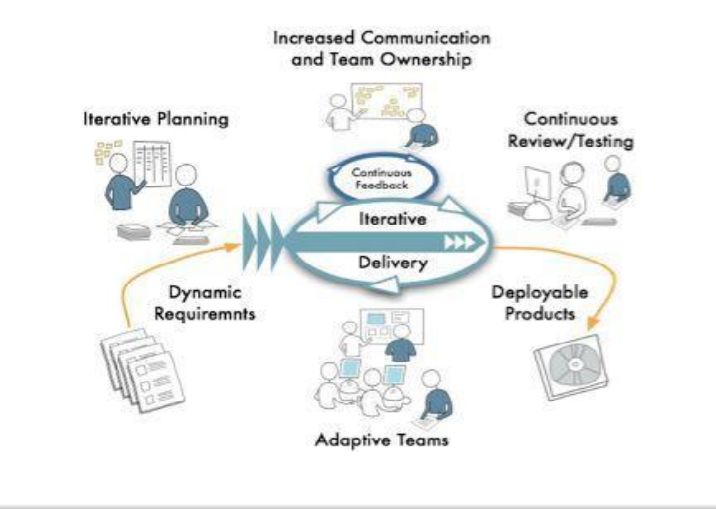
\includegraphics[width=5in]{agile1.png} 
\vspace{.1cm}
\chapter{Literature Survey}

\paragraph{}
\large\textnormal{Magpy is a web data extraction tool which uses the concept of web scraping and crawling. The most popular seach engines available are Google ,Yahoo and Bing. Google Search, commonly referred to as Google Web Search or just Google, is a web search engine owned by Google Inc. It is the most-used search engine on the World Wide Web, handling more than three billion searches each day.Yahoo! is an Internet portal that incorporates a search engine and a directory of World Wide Web sites organized in a hierarchy of topic categories. As a directory, it provides both new and seasoned Web users the reassurance of a structured view of hundreds of thousands of Web sites and millions of Web pages.Since Yahoo is associated with the most popular Web search sites, if a search argument doesn't lead to a Yahoo topic page, it will still lead to results from the six or seven popular search engine sites Yahoo links to.Bing is a search engine created and operated by Microsoft, replacing its former Live Search, Windows Live Search, and MSN Search offerings.Bing takes into account  more than 1 000 signals to order websites on search engine result pages.}

\paragraph{}
\large\textnormal{Eventhough these search engines provide so many features but they  donot support the constraints based searching. For example, we are not able to use negative keywords, search by using regular expressions, search for only required block of contents etc. Even though the existing search engines have got searching based on the type of documents needed, the availability of this facility is known only to a certain class of people.}

\paragraph{}
\large\textnormal{The existing search engines do not provide extra facilities like being able to filter passages of specific sizes, highlight the updations that has occurred within a certain amount of time, or customized search like for example being able to show only results having articles and relevant images. But by using MagPy the users are given the power to do all these, in a simple and user friendly interface. Along with these functionalities, MagPy also provides a bunch of other constraints that are not present in the current system, or are not easy to implement. With top results extracted from top search engines like Google, Bing and Yahoo, the results provided by MagPy are comparatively more efficient than the results provided by any search engine alone. Another case is that where the user needs to search for contents semantically, as the example of kingfisher. The user can simply specify a negation of the term airlines to imply that what the user needs is not about kingfisher airlines, but about the bird.}

\paragraph{}
\large\textnormal{Taking into consideration the working of present search engines and crawlers, they work on the basis of the metadata like description, tags, SEO tips and keywords that are provided by the website creator. This can be a disadvantage if “keyword stuffing” or similar technique is used to fool the search engine, and be on top of their results. But MagPy does the job of further drilling down into the page and filtering the real and fake pages out.Also, with a system to watch a webpage for certain updates and with the ability to provide data from just targeted section of the page, MagPY improves the speed, accuracy and reduces the burden of the user to a large extent.}

\paragraph{}
\large\textnormal{This product is designed as a desktop application, coupled with apps for smartphones, that is targeted to any kind of audience and does the task of enhancing the quality and way the user searches the web, using various constraints and actions. It includes many constraints, website update checkers, filters and quick links, enabling user to do tasks that are either not possible to do with the existing search engines, or are not possible directly. With all these inbuilt, the product will be designed to use minimal amount of resources and will be capable of running smoothly with low hardware devices also.}

\paragraph{}
\large\textnormal{The final product is intended to work on any common system running Windows, Linux, Android, Windows Phone or iOs, without any special external support. Along with the client apps, there is a central server that is mainly used for collecting the query results from different users and use them to refine the filtering techniques, providing a continuous improvement of the results through automatic studying. So the only interface requirement would be the common server we intend to host.}

\paragraph{}
\large\textnormal{In brief, this project is focused on producing a web based document extraction tool presented in a simple GUI, and provides the capabilities to search using keywords and regular expressions, and along with it, constrain the results based on different criteria. It acts as an advancement over the modern search engines by providing the capability to filter results and partial load web pages for contents or peek into the web pages, which is not possible in the current scenario..}

\paragraph{}
\large\textnormal{The existing search engines do not provide extra facilities like being able to filter passages of specific sizes, highlight the updations that has occurred within a certain amount of time, or customized search like for example being able to show only results having articles and relevant images. But by using MagPy the users are given the power to do all these, in a simple and user friendly interface.}

\paragraph{}
\large\textnormal{Taking into consideration the working of present search engines and crawlers, they work on the basis of the metadata like description, tags, SEO tips and keywords that are provided by the website creator. This can be a disadvantage if “keyword stuffing” or similar technique is used to fool the search engine, and be on top of their results.}

\chapter{Hardware and Software Specifications}
\paragraph{}
\large\textnormal{There are no major external components involved in the development of this project. The components of the software itself are only the server and the client apps.}
\large\textnormal{The hardware and software requirements for the user to use the final 
product are as follows:}
\section{Hardware}


\textbf{PC users:}

Minimum 1 gigahertz (GHz) or faster 32-bit (x86) or 64-bit (x64) processor 256 MB of RAM.\newline
\textbf{Mobile Users:}

Minimum 800 Megahertz (MHz) or faster processor 100 MB of RAM

\section{Software}


\textbf{PC Users:}

Python pre-installed.\newline
\textbf{Mobile Users:}

None.

\chapter{System Analysis and Design}

\section{Existing System}
\paragraph{}
\large\textnormal{Current web search experience experiences a lot of drawbacks including the inability to use constraints in the search results, like to negate a keyword, limit the size of results, or to provide only results having a specified size, target only specific region of the result page rather than loading the whole page for viewing just a small portion of it and so on.The current web search engines also lack the feature of automation.}
\paragraph{}
\large\textnormal{If we want to obtain some web data for analysis, we need to manually go through the results from search engines or multiple sources. So it involves a great amount of time and effort. Since a lot of data had been retrieved from the web the bandwidth consumed will also be huge.  The order in which the data has to be organized for analysis has great importance. By using the current system the organization of data is a very hectic task. Our simplified web extraction system, MagPY is a solution to all existing problems that we have encountered.}
\section{Requirement Analysis}
\paragraph{}
\large\textnormal{The analysis of currently available search engine lead us to the requirement of an automated web data extraction tool or system that can extract only the necessary data from web instead of flooding with a large amount of unnecessary information’s. This requirement lead to the design of a web data extraction and processing tool by providing capabilities to navigate through multiple web pages, collect relevant data, process it and export it into user-specified formats. With the ability to filter search results using various constraints, watch website updates and automate web based activities. Since a huge amount of data has been loaded to the client side, the bandwidth also increases to a large extent. MagPY provides an answer to this requirement and hence reduces the time and effort in transferring data.In short this made to the origin of our project MagPY which aims at changing the way users search for content in the web and to bring a revolution in the way users approach the World Wide Web.}

\section{Proposed System}
\paragraph{}
\large\textnormal{MagPY is a web data extraction system capable of providing an interface to gather data that shifts the burden of loading pages to server and reducing the bandwidth. This will reduce the time as well as the effort required in transferring the data from server to client. Thus by lightening the processes at client side. It help us to navigate through multiple web pages based on search results in search engines, iterations and regular expressions. This enables the users to search for their required results. The multi-level selection and filtering power in order to target a specific element in a web page or multiple web pages is the main facility of MagPY. There are multi-format options that help us in keeping the results in organized manner. The main attraction of the system is that it provides a data watcher and the remote server manager facility called MyVault. The user will get the data at their personal PC which will be downloaded in some other systems. This project provides a tool capable of multiple document extraction options like text, images, videos and other files. There are multiple filtering, navigation and automation options available by simplifying the process to just a few clicks.}

\section{Module Division}
\subsection{Module 1}
\large\textnormal{This module is handled by Thumssy P. Nazar which includes Web navigator,non-textual data processing and MyVault System.}
\subsubsection{Web navigator}
\large\textnormal{This involves crawling through multiple pages as per user specification and collecting data from them.}
\subsubsection{Non-textual data processing}
\large\textnormal{This involves grabbing and filtering non-textual data like images, videos, pdfs or other file types.}
\subsubsection{MyVault}
\large\textnormal{This involves managing the accounts and managing the synchronization between connected systems.}
\subsection{Module 2}
\large\textnormal{This module is handled by Sarath S Menon which includes data processing, export mechanisms and MyVault account management.}
\subsubsection{Data Processing}
\large\textnormal{Involves filtering and processing of textual data from web pages.}
\subsubsection{Export Mechanisms}
\large\textnormal{Involves exporting available data to docx, pdf, xml, excel, csv, json, txt etc.}
\subsubsection{MyVault Account Manager}
\large\textnormal{Involves managing the accounts and device sync in MyVault.}
\subsection{Module 3}
\large\textnormal{This module is handled by Sarath S Menon which includes GUI, MyVault web and MagPY application.}
\subsubsection{GUI}
\large\textnormal{Involves all the graphical user interface elements for interacting with the user and the server.}

\subsubsection{MyVault Web}
\large\textnormal{Involves managing the web interface of the MyVault mechanism, adding remote administration tools.}

\subsubsection{MyVault Application}
\large\textnormal{Involves development of an app, making the tool portable.}
\newpage


\begin{figure}
\section{DFDs and UML diagrams}
\paragraph{}
\large\textnormal{The project architecture can be represented as follows:}
\vspace{.3cm}
\center
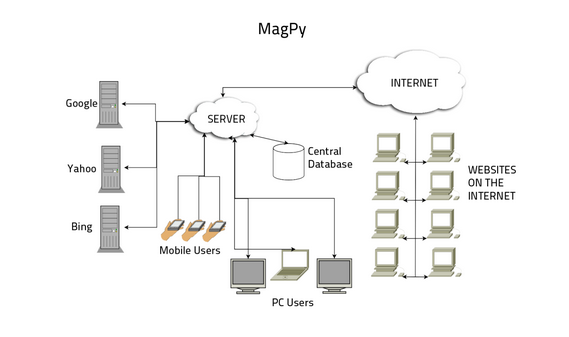
\includegraphics[width=6in]{architecture.png} 
\vspace{.3cm}
\end{figure}

\paragraph{}
\large\textnormal{The primary objective of this project is to provide a better search experience, so the initial system function would be the Search itself. The search functionality provides an interface for the user to enter the keywords on the basis of which the search is to be done, along with an interface to enter the constraints that are to be applied to the resulting data, so that the exact content is obtained, rather than obtaining links to possibly correct contents, as in the case of current search engines.} 

\center
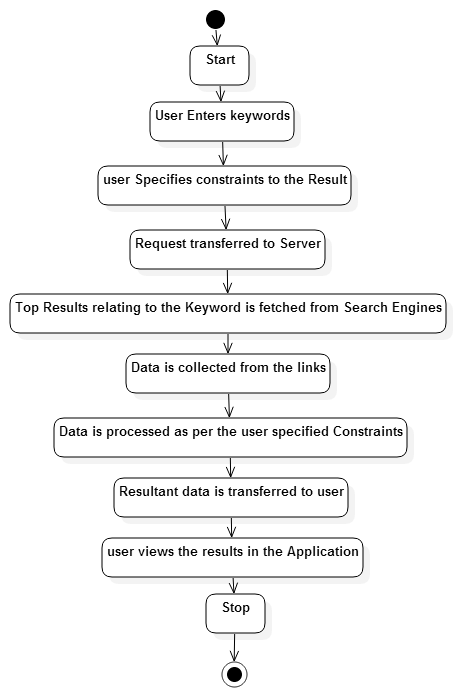
\includegraphics[width = 5in]{SearchActivity.png}  
\newpage


\begin{figure}
\paragraph{}
\large\textnormal{The second system functionality implemented by this system is the “watch” functionality, which provides the ability to watch websites and specific pages or sections for updates over a period of time.The “watch” module is targeted at providing an interface where the system can be made to “watch” a page or a portion of a page for updates over time. It starts when the user specifies the page or the portion of the page where the system has to “watch”. Once the details are obtained, the system continuously monitors the page or portion using the “PING” system. This “PING” system checks updates at regular intervals, which can be modified by the user.}
\center
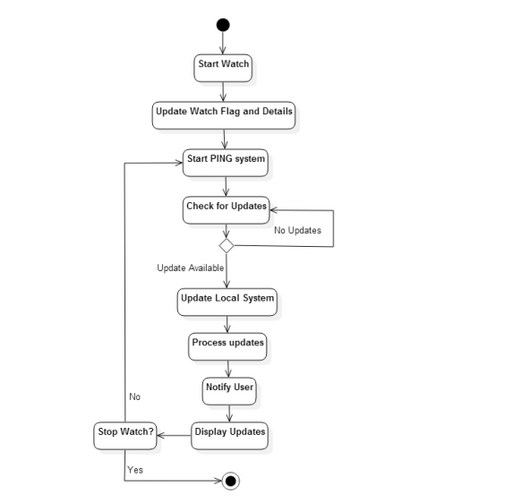
\includegraphics[width=5in]{watchdfd.png} 
\end{figure}


\newpage
\begin{figure}
\paragraph{}
\large\textnormal{The next system functionality implemented by this system is the feature named “MyVault”. It is an advanced system that provides the capability to remotely save files and process data into a special storage space allotted to each user, called MyVault. This allows dynamic syncing of files and remote file download capabilities. This module of this system can be visualized as an interface which can be accessed from any remote system by providing a user authentication. The user can add links to be viewed later, or downloaded onto the user’s local system or another device that the user has registered with this service. By simply providing the link, the file will automatically be downloaded and synced to the various devices, and if it it is a read-later link, the user will be notified once he uses his system, about the link, which will be downloaded, so that the user can view it offline.}
\end{figure}
\newpage
\begin{figure}
\center

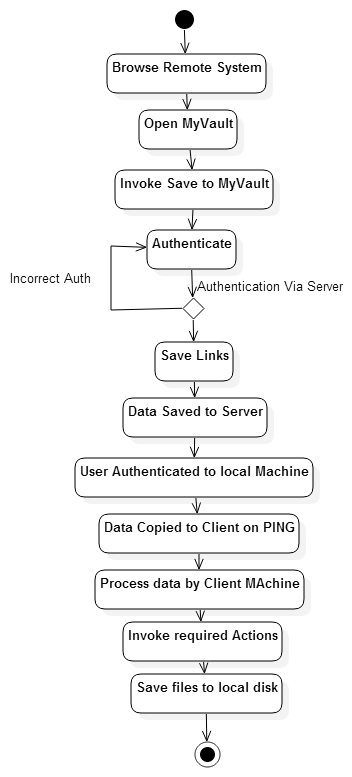
\includegraphics[width=4in]{MyVault_Activity.png}
\end{figure}
 

\chapter{Implementation}
\chapter{Testing Strategies}
\chapter{Results}
\chapter{Discussion}
\chapter{Conclusion}
\chapter{Future Enhancement}
\chapter{References}
\chapter{Appendices}















\end{document}
\end